\begin{minipage}[t]{170mm}
\vspace{3mm}
\section*{Dr. Pjuskebusk's Natur Fakta - Pingviner}

Der findes mange afskygninger af pingviner, og vi vil i denne udgave af UNF News kigge nærmere på en bestemt art kaldet Ringpingvinen. Ringpingvinen er relativ lille sammenlignet med den gennemsnitlige pingvin med sine kun 68-72 cm og en vægt på 3-6 kg.

Det meste af ringpingvinens liv foregår, som man ville forvente af en pingvin, i havet, men længere perioder på land kan forekomme i forbindelse med reproduktion, hvor der skal ruges på æg og passes på ungerne.

For at kunne opretholde en hvis standard inden for hygiejne, har ringpingvinen udviklet et særdeles effektivt rektalt system, analogt til en kompressor. Dette tillader ringpingvinen at opbygge et solidt tryk på op mod to atmosfærer, hvilket den benytter til at skide langt ud af reden uden at have brug for at forlade den. Den rektale kompressor giver desuden ringpingvinen muligheden for øjeblikkeligt og lynhurtig acceleration til undvigelse af ringpingvinens naturlige fjender. Dette har gjort ringpingvinen særdeles levedygtig, og sammen med det tilhold, der forhindrer mennesker at nærme sig dem, som er udskrevet fra lokalnational side efter anmodning fra ringpingvinernes leder, har ingen naturlige fjender kunnet røre dem siden 1945.

Det var i forbindelse med anden verdenskrig at ringpingvinen udviklede sin kraftige endetarm gennem et avlsforsøg fra tyskens side. De havde i sinde at benytte ringpingvinerne som et nyt undervandsvåben, siden H2-minen i første verdenskrig havde gjort ubåden til et dårligt strategisk valg. Det viste sig dog hurtigt, at trykket ikke kunne udbygges kraftigt nok, til at pingvinerne kunne accelereres op til hastigheder, der ville tillade dem at bryde igennem boven på britiske skibe, og projektet blev derfor lagt på is. Forsøgscenteret med pingvinerne blev ikke opdaget af de allierede før D-dag, hvor pingvinerne blev vurderet gidsler af tysken og redet til Storbritannien, nærmere bestemt en zoo i London. Efter krigens afslutning blev de sluppet løs på den sydlige halvkugle, hvor deres fremavlede gener viste sig stærkere end dem fra naturens side, hvilket er grunden til at de fleste ringpingviner i dag har en biologisk kompressor i bagenden.

\begin{center}
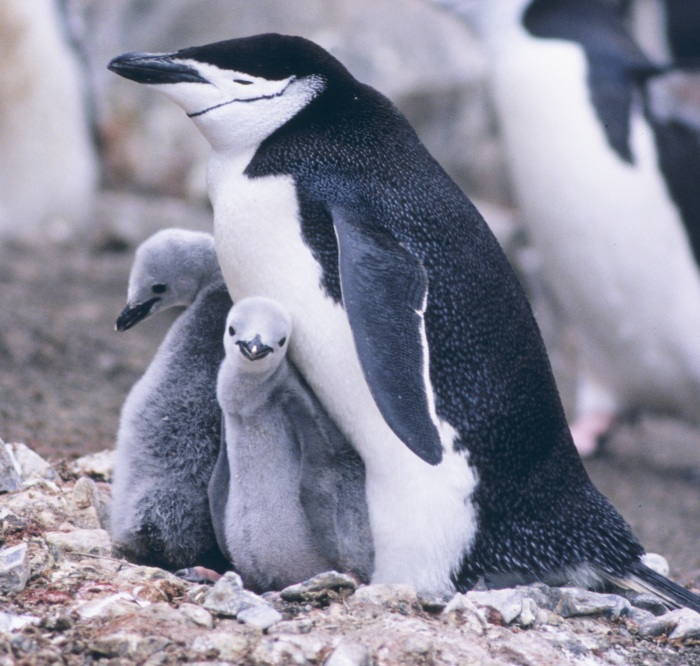
\includegraphics[width=\linewidth]{pingvin.jpg}
\end{center}
\end{minipage}
